\section{Analog Front-End and ADC}

The analog front-end of the 4-channel ADC module is organized as two-stage chain that conditions each video input before digitalization. \autoref{fig:front_end_adc} illustrates the complete signal path for a single video channel. First, a low-noise instrumentation amplifier provides a well-defined return path, input impedance and gain for the input differential signal from detector. Second, a Fully Differential amplifier implements a low-pass filter and sets common-mode voltage for ADC. And finally, a high-speed SAR ADC samples the video signal and send data to Zynq SoC through \SI{2.5}{\volt} LVDS.

\begin{figure}[ht]
  \centering
  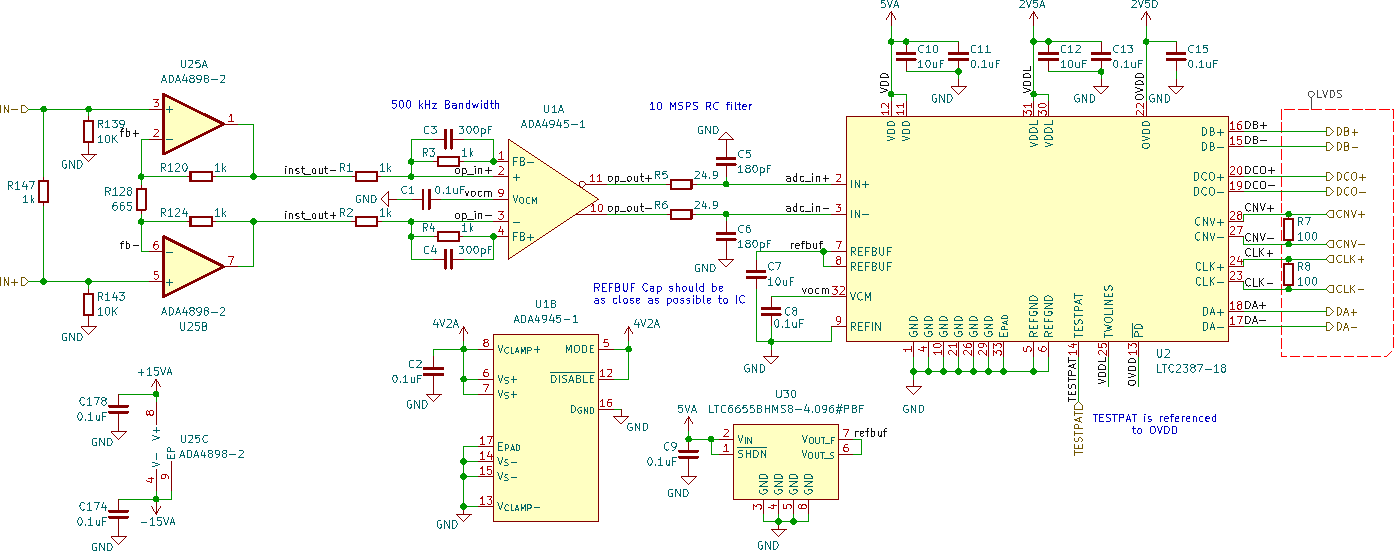
\includegraphics[width=1\linewidth]{sections/front_end_adc/fig_front_end_adc.pdf}
  \caption{Analog Front-End and ADC Circuit.}
  \label{fig:front_end_adc}
\end{figure}

Using Analog Devices Signal Chain Designer, the total noise refered to the input from \SI{0.1}{\hertz} to \SI{5}{\mega\hertz} is \SI{12.9}{\micro\volt_{rms}}, where:

\begin{itemize}
    \item Instrumentation amplifier: \SI{2.94}{\micro\volt_{rms}}.
    \item Fully differential amplififer: \SI{3.52}{\micro\volt_{rms}}.
    \item ADC: \SI{12}{\micro\volt_{rms}}.
\end{itemize}

Referred to front-end input:
\begin{itemize}
  \item Input signal swing: $v_\text{in}^\text{max} = 8.192/4 = \SI{2.05}{\volt}$ (DC gain of \SI{4}{\volt/\volt} and ADC input range of \SI{8.192}{\volt}).
  \item AC max signal: $v_\text{in,AC}^\text{max} = v_\text{in}^\text{max}/2/\sqrt{2} = \SI{723}{\milli\volt_{rms}}$.
  \item Signal chain noise: $n_\text{in} = \SI{12.9}{\micro\volt_{rms}}$.
  \item The Signal-to-Noise ratio (SNR): $20\log_{10}(v_\text{in,AC}^\text{max}/n_\text{in}) = \SI{94.99}{\decibel}$.
  \item Effective-Number-of-Bits (ENOB) without distortion: $(\text{SNR} - 1.76)/6.02 = \SI{15.49}{\bit}$.
\end{itemize}

\subsection{Instrumentation Amplifier}

\autoref{fig:inst_amp} shows the two opamp instrumentation amplifier equivalent circuit. Resistor $R_1=\SI{1}{\kilo\ohm}$ and $R_2=\SI{10}{\kilo\ohm}$ define input impedance, common mode path and return path for video input. Output common-mode voltage is maintaned and differential gain $G_1$ is set by $R_3 = \SI{665}{\ohm}$ and $R_4 = \SI{1}{\kilo\ohm}$ $\pm$\SI{0.1}{\percent} as:

\begin{equation}
    G_1 \equiv \frac{v_\text{out}}{v_\text{in}} =\frac{{v_\text{out}^+-v_\text{out}^-}}{v_\text{in}^+-v_\text{in}^-}= 1+\frac{2R_4}{R_3} \approx \SI{4}{\volt/\volt}
\end{equation}

\begin{figure}[ht]
  \centering
  \begin{tikzpicture}[scale=0.75, transform shape]
    
    \draw (0,0) node[circ]{} coordinate(R3bot) to[R, l=$R_3$] ++(0,2) node[circ]{} coordinate (R3top);

    \draw (R3top) -- ++(0,1) node[op amp, yscale=-1, anchor=-] (A1){};
    \draw (R3bot) -- ++(0,-1) node[op amp, yscale=1, anchor=-] (A2){};

    \draw (A1.+) to[short,-*] ++(-2,0) coordinate (R1top);
    \draw (A2.+) to[short,-*] ++(-2,0) coordinate (R1bot);

    \draw (R1top) to[R, l=$R_2$] ++(0, 2) node[ground, yscale = -1]{};
    \draw (R1bot) to[R, l=$R_2$] ++(0, -2) node[ground]{};
    \draw (R1top) to[R, l_=$R_1$] (R1bot);

    \draw (R1top) -- ++(-1,0) node[ocirc]{} node[left]{$v_\text{in}^+$};
    \draw (R1bot) -- ++(-1,0) node[ocirc]{} node[left]{$v_\text{in}^-$};

    \coordinate (aux1) at (R3top -| A1.out);
    \coordinate (aux2) at (R3bot -| A2.out);

    \draw (R3top) to[R, l_=$R_4$] (aux1) -- (A1.out) node[circ]{} -- ++(0.5,0) node[ocirc]{} node[right]{$v_\text{out}^+$};
    \draw (R3bot) to[R, l^=$R_4$] (aux2) -- (A2.out) node[circ]{} -- ++(0.5,0) node[ocirc]{} node[right]{$v_\text{out}^-$};

\end{tikzpicture}
  \caption{Instrumentation Amplifier Equivalent Circuit.}
  \label{fig:inst_amp}
\end{figure}

For instrumentation amplifier we selected the Analog Devices ADA4898-2 dual operational amplifier that features:
\begin{itemize}
    \item Ultralow voltage noise: \SI{0.9}{\nano\volt/\sqrtunit{\hertz}} and \SI{2.4}{\pico\ampere/\sqrtunit{\hertz}} at \SI{1}{\kilo\hertz}.
    \item Ultralow distortion: \SI{-93}{\decibel c} at \SI{500}{\kilo\hertz}.
    \item High speed: \SI{65}{\mega\hertz} bandwidth at unity gain.
    \item Unity gain stable.
    \item Low input offset: \SI{160}{\micro\volt} maximum.
\end{itemize}

\subsection{Fully Differential Amplifier}

\autoref{fig:fda} shows the fully differential circuit equivalent circuit. Resistors $R_1=R_2=\SI{1}{\kilo\ohm}$ $\pm$ \SI{0.1}{\percent} define input impedance and differential gain. Output common-mode voltage is set externally by ADC to \SI{2.048}{\volt} and differential gain $G_2$ is set as:

\begin{equation}
    G_2 \equiv \frac{v_\text{out}}{v_\text{in}} =\frac{{v_\text{out}^+-v_\text{out}^-}}{v_\text{in}^+-v_\text{in}^-}= \frac{R_2}{R_1} = \SI{1}{\volt/\volt}
\end{equation}

The bandwidth BW is defined by $R_2$ and $C_1=\SI{300}{\pico\farad}$ for \SI{1}{\mega SPS} as:

\begin{equation}
    \text{BW} = \frac{1}{2\pi R_2 C_1} \approx \SI{530}{\kilo\hertz}
\end{equation}

\begin{figure}[ht]
  \centering
  \begin{tikzpicture}[scale=0.75, transform shape]
    
    \draw (0,0) node[fd op amp] (opamp){};

    \draw (opamp.-) node[circ]{} -- ++(0,1) coordinate(opintop) node[circ]{};
    \draw (opamp.+) node[circ]{} -- ++(0,-1) coordinate(opinbot) node[circ]{};

    \draw (opamp.-) to[R, l_=$R_1$] ++(-2,0) node[ocirc]{} node[left]{$v_\text{in}^-$};
    \draw (opamp.+) to[R, l=$R_1$] ++(-2,0) node[ocirc]{} node[left]{$v_\text{in}^+$};

    \draw (opintop) to[R, l=$R_2$] (opintop -| opamp.out +) node[circ]{} -- (opamp.out +) node[circ]{};
    \draw (opinbot) to[R, l_=$R_2$] (opinbot -| opamp.out -) node[circ]{} -- (opamp.out -) node[circ]{};

    \draw (opintop) node[circ]{} -- ++(0,1.25) coordinate(rtop);
    \draw (opinbot) node[circ]{} -- ++(0,-1.25) coordinate(rbot);
    
    \draw (rtop) to[C, l=$C_1$] (rtop -| opamp.out +) -- (opintop -| opamp.out +);
    \draw (rbot) to[C, l_=$C_1$] (rbot -| opamp.out -) -- (opinbot -| opamp.out -);

    \draw (opamp.out +) -- ++(0.5,0) node[ocirc]{} node[right]{$v_\text{out}^+$};
    \draw (opamp.out -) -- ++(0.5,0) node[ocirc]{} node[right]{$v_\text{out}^-$};


\end{tikzpicture}
  \caption{Fully Differential Amplifier Equivalent Circuit.}
  \label{fig:fda}
\end{figure}

As fully differential amplifier we selected the Analog Devices ADA4945-1 in full-power mode that features:

\begin{itemize}
    \item Rail-to-rail output.
    \item \SI{4}{\milli\ampere} at full-power mode.
    \item \SI{145}{\mega\hertz} bandwidth at gain 1 at full-power mode.
    \item Low noise: \SI{2}{\nano\volt/\sqrtunit{\hertz}} at \SI{100}{\kilo\hertz}.
    \item \SI{115}{\micro\volt} maximum offset voltage.
\end{itemize}

\subsection{Analog-to-Digital Converter (ADC)}

\autoref{fig:filter} shows ADC input filter equivalent circuit. For an \SI{18}{\bit}, the error of a full scale range (FS) step in a single-pole $RC$ filter after acquisition time $t_\text{ACQ}$ is $\exp\left(-\frac{t_\text{ACQ}}{R_\text{filt}C_\text{filt}}\right)\text{FS}$ and a half LSB is approximately $2^{-19}\, \text{FS}$. Then we have

\begin{equation}
    \exp\left(-\frac{t_\text{ACQ}}{R_\text{filt}C_\text{filt}}\right)\text{FS} = 2^{-19}\,\text{FS} \Leftrightarrow C_\text{filt} = \frac{t_\text{ACQ}}{19R_\text{filt}\ln 2}
\end{equation}

\begin{figure}[ht]
  \centering
  \begin{tikzpicture}[scale=0.75, transform shape]
    
    \draw (0,0) node[ocirc]{} node[left]{$v_\text{in}^+$} to[R, l=$R_\text{filt}$] ++(2,0) node[circ]{} coordinate(rtop){} -- ++(0.5, 0) node[ocirc]{} node[right]{{$v_\text{out}^+$}};

    \draw (0,-1) node[ocirc]{} node[left]{$v_\text{in}^-$} to[R, l_=$R_\text{filt}$] ++(2,0) node[circ]{} coordinate(rbot){} -- ++(0.5, 0) node[ocirc]{} node[right]{{$v_\text{out}^-$}};

    \draw (rtop) to[C, l_ = $C_\text{filt}$] ++(0,2) node[ground, yscale = -1]{};
    \draw (rbot) to[C, l = $C_\text{filt}$] ++(0,-2) node[ground, yscale = 1]{};

\end{tikzpicture}
  \caption{ADC Input filter Equivalent Circuit.}
  \label{fig:filter}
\end{figure}

We selected the Analog Devices LTC2387-18 \SI{18}{\bit} \SI{15}{\mega S P S} SAR ADC that features:

\begin{itemize}
    \item No pipeline delay, no cycle latency.
    \item \SI{95.7}{\decibel} SNR at \SI{1}{\mega\hertz}.
    \item \SI{102}{\decibel} SFDR at \SI{1}{\mega\hertz}.
    \item $\pm$\SI{3}{LSB} INL maximum.
    \item \SI{8.192}{\volt_{p-p}} differential input.
    \item \SI{2.5}{\volt} Serial LVDS interface.
\end{itemize}

For selected ADC we have $t_\text{ACQ} = 1/f_s -\SI{39}{\nano\second}$. For $f_s = \SI{10}{\mega SPS}$ sample rate and $R_\text{filt}=\SI{24.9}{\ohm}$ we get $C_\text{filt}\approx \SI{180}{\pico\farad}$.

To improve ADC reference voltage temperature drift,  reference out pin (\texttt{REFBUF}) is externally driven by Analog Devices LTC6655 \SI{4.096}{\volt} low drift voltage precision reference that features:

\begin{itemize}
  \item Low Noise: \SI{0.25}{ppm_{P-P}} (\SI{0.1}{\hertz} to \SI{10}{\hertz}).
  \item Low drift: \SI{2}{ppm/\degreeCelsius}.
  \item High accuracy: $\pm$\SI{0.025}{\percent} maximum.
  \item Long term drift: \SI{20}{ppm /\sqrtunit{\kilo\hour}}.
\end{itemize}